\documentclass[12pt]{article}

\usepackage{tabularx}
\usepackage[table]{xcolor}
\usepackage{multirow}

\usepackage{amsmath, amssymb}
\usepackage{mathtools}

\usepackage{listings}

\usepackage{tikz}
\usetikzlibrary{positioning}
\usetikzlibrary{patterns}
\usetikzlibrary{matrix,backgrounds}
\usetikzlibrary{arrows,shapes,trees}
\usetikzlibrary{chains,shapes}
\usetikzlibrary{arrows}
\usetikzlibrary{decorations.pathmorphing}

\usepackage[siunitx, RPvoltages]{circuitikz}

%\usepackage{pst-coil}

\usepackage[margin=1.1in,footskip=.25in]{geometry}

\usepackage[most]{tcolorbox}

\tcbset{
    frame code={}
    center title,
    left=10pt,
    right=10pt,
    top=10pt,
    bottom=10pt,
    colback=gray!5,
    colframe=gray,
    width=\dimexpr\textwidth\relax,
    enlarge left by=0mm,
    boxsep=5pt,
    arc=0pt,outer arc=0pt,
}




\newcommand*{\thread}{
\begin{circuitikz}[
 longpot/.style = {R, resistors/scale=0.75,
 resistors/width=1.6, resistors/zigs=6}]
 \draw (0,0) to[longpot] ++(0,-3);
\end{circuitikz}
}


\newcommand*{\threadsmall}{
\begin{circuitikz}[
 longpot/.style = {R, resistors/scale=0.5,
 resistors/width=1, resistors/zigs=6}]
 \draw (0,0) to[longpot] ++(0,-1);
\end{circuitikz}
}

\begin{document}


\section{Operating System}

\begin{itemize}
	\item Process
	\item Threads
	\item CPU Scheduling
	\item Process Synchronization
	\item Dead Locks
	\item Memory Management
	\item Virtual Memory
	\item File System
	\item I/O System
	\item Disk Management
	\item Protection
	\item Security
\end{itemize}




\section{Process}


\begin{itemize}
	\item a program in execution
	\item an asynchronous activity
	\item manifested by Process Control Block
	\item Entity to which processor can be assigned
	\item the dispatchable unit
\end{itemize}




\section{Process Table}



\begin{center}
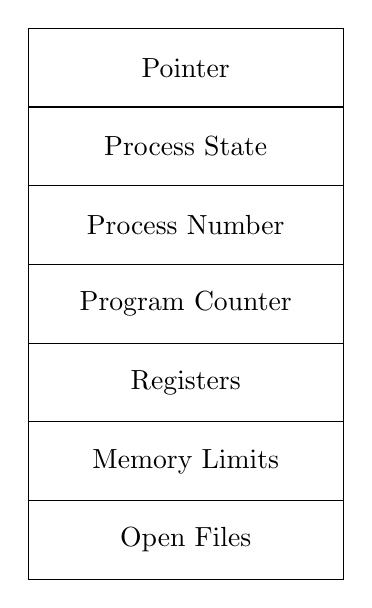
\begin{tikzpicture}
\draw (0,0) rectangle (4,-1);
\draw (0,-1) rectangle (4,-2);
\draw (0,-2) rectangle (4,-3);
\draw (0,-3) rectangle (4,-4);
\draw (0,-4) rectangle (4,-5);
\draw (0,-5) rectangle (4,-6);
\draw (0,-6) rectangle (4,-7);

\node[scale=1] at (2,-0.5) {Pointer};
\node[scale=1] at (2,-1.5) {Process State};
\node[scale=1] at (2,-2.5) {Process Number};
\node[scale=1] at (2,-3.5) {Program Counter};
\node[scale=1] at (2,-4.5) {Registers};
\node[scale=1] at (2,-5.5) {Memory Limits};
\node[scale=1] at (2,-6.5) {Open Files};
\end{tikzpicture}
\end{center}





\section{Process State Transition}





\section{Threads}


\begin{itemize}
	\item Single Sequence Stream within a Process
	\item Processes are used to group resources together and threads are the entities scheduled for execution on the CPU
\end{itemize}




\section{Threads - Advantages}


\begin{itemize}
	\item Responsiveness
	\item Resource Sharing
	\item Economy
	\item Utilization of MultiProcessors Architectures
\end{itemize}





\begin{center}
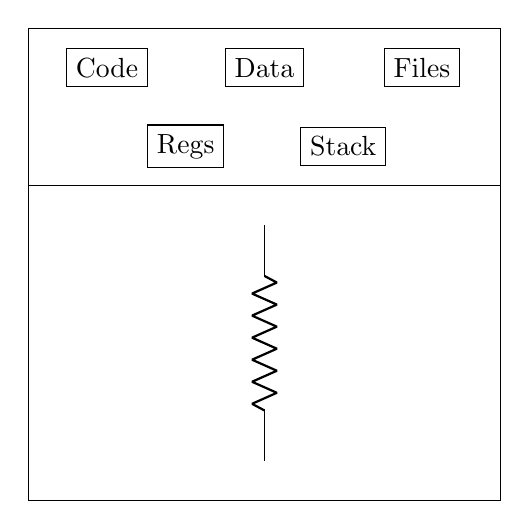
\begin{tikzpicture}
\draw (0,0) rectangle (6,-2);
\draw (0,-2) rectangle (6,-6);
\node[draw] at (1,-0.5) {Code};
\node[draw] at (3,-0.5) {Data};
\node[draw] at (5,-0.5) {Files};
\node[draw] at (2,-1.5) {Regs};
\node[draw] at (4,-1.5) {Stack};

\node at (3,-4) {\thread};
\end{tikzpicture}
\end{center}





\begin{center}
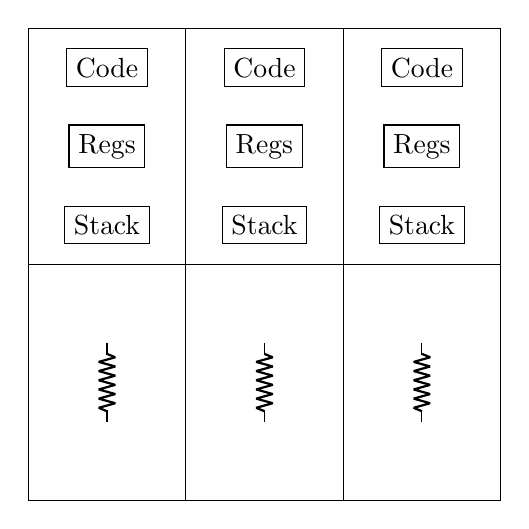
\begin{tikzpicture}
\draw (0,0) rectangle (6,-3);
\draw (0,-3) rectangle (6,-6);

\draw (0,0) rectangle (2,-6);
\draw (2,0) rectangle (4,-6);

\node[draw] at (1,-0.5) {Code};
\node[draw] at (1,-1.5) {Regs};
\node[draw] at (1,-2.5) {Stack};

\node[draw] at (3,-0.5) {Code};
\node[draw] at (3,-1.5) {Regs};
\node[draw] at (3,-2.5) {Stack};

\node[draw] at (5,-0.5) {Code};
\node[draw] at (5,-1.5) {Regs};
\node[draw] at (5,-2.5) {Stack};



\node at (1,-4.5) {\threadsmall};
\node at (3,-4.5) {\threadsmall};
\node at (5,-4.5) {\threadsmall};
\end{tikzpicture}
\end{center}








\section{CPU Scheduler}


\begin{itemize}
	\item Select a process for execution and allocate CPU
\end{itemize}


Scheduling Decision will require following Transitions :

\begin{itemize}
	\item running $\to$ waiting
	\item running $\to$ ready
	\item waiting $\to$ ready
	\item terminate
\end{itemize}





\section{Scheduling Types}

\begin{itemize}
	\item pre-emptive : 
	I shall not take CPU from a process untill it release that process
	\item non pre-emptive :
	I can take CPU from process if such priority demands
\end{itemize}



\section{General goals of CPU Scheduling}


\begin{itemize}
	\item Fairness
	\item Policy Enforcements
	\item Efficiency
	\item Response-Time
	\item Turn Around Time
	\item Thoughtput 
\end{itemize}





\section{Dispatcher}

The dispatcher should be as fast as possible, since it is invoked in every process switch .
\newline\newline
\noindent
dispatch latency should be minimum .




\section{Scheduling Criteria}



\begin{itemize}
	\item CPU Utilization
	\item Thoughput ( number of processes completed per unit time )
	\item Turn Around time ( the time between the submission and completion )
	\item waiting time
	\item response time
\end{itemize}






\section{CPU Scheduling - Scheduling Types}


\begin{itemize}
	\item FCFS Scheduling
	\item SJF Scheduling
	\item Priority Scheduling
	\item Round-Robin Scheduling
	\item Multi-Level Queue Scheduling
	\item Multi-Level Feedback Queue Scheduling 
\end{itemize}





\section{Process Synchronization-Critical Section Problem}

A Solution to the Critical Section Problem must satisfy the following three requirements .

\begin{itemize}
	\item Mutual Exclusion
	\item Progress
	\item Bounded Waiting
\end{itemize}


\noindent
Mutual Exclusion $\xRightarrow{\text{means}}$ in the critical section at a time one and only one process can get an entry .
\newline\newline
\noindent
Bounded Waiting $\xRightarrow{\text{means}}$ Process \textbf{X} requesting to enter the critical section and another Process \textbf{Y} is entering critical section too , how many times Process \textbf{X} should denied should have UpperLimit and that Knows as \textbf{Bounded Waiting}






\section{DeadLock}


A Process or thread is in the state deadlock if it is waiting for a particular event that will not occur .



\end{document}